\chapter{Git}
Git é o atual \textit{state-of-the-art} sistema de controle de versão e tem sido
utilizado em vários projetos, muitos na área de desenvolvimento de software,
sendo o grande destaque o Kernel Linux. Este modelo de tese possui suas versões
controladas por meio do Git e na próxima sessão será apresentado algumas
dicas de como utilizar o Git para aproveitar melhor este modelo por meio da
linha de comando e na sessão seguinte pela interface gráfica nativa do Git.

\section{Pela linha de comando}
\subsection{Baixando o modelo}
Para baixar o modelo utilizando o Git você deve executar o comando:
\begin{lstlisting}[escapechar=@]
$ git clone https://github.com/r@-@gaia@-@cs/modelo_tese_imecc.git
\end{lstlisting}
Será criado uma pasta \lstinline+modelo_tese_imecc+ com os arquivos do
modelo.

Além da versão oficial do modelo existem algumas outras e para ver uma lista
destas versões você deve executrar o comando:
\begin{lstlisting}
$ git branch
\end{lstlisting}
Para selecionar a versões a ser utilizada, execute o comando:
\begin{lstlisting}
$ git branch versao_desejada
\end{lstlisting}
A versão oficial é chamada de \lstinline+master+.

Antes de começar a editar os arquivos, execute os comandos:
\begin{lstlisting}
$ git branch meu_trabalho
$ git checkout meu_trabalho
\end{lstlisting}

\subsection{Editando o modelo}
Evite ao máximo modificar os arquivos originais do modelo pois isso facilitará a
atualização do mesmo como será apresentado na seção seguinte.

Para adicionar novos arquivos ao controle de versão, execute o comando:
\begin{lstlisting}
$ git add novo_arquivo
\end{lstlisting}
E para adicionar modificações nos arquivos previamente adicionados ao controle
de versão, execute o comando:
\begin{lstlisting}[escapechar=@]
$ git add @-@u
\end{lstlisting}

Para criar uma nova versão da sua dissertação/tese, execute o comando:
\begin{lstlisting}[escapechar=@]
$ git commit @-@m 'Breve descricao do que foi feito ate agora.'
\end{lstlisting}

\subsection{Atualizando o modelo}
Como este modelo é um trabalho em progresso e não existe nenhuma garantia de que
as deliberações da Comissão Central de Pós-Graduação serão mantidas até que você
termine seu mestrado/doutorado é importante existir uma maneira de você
atualizar sua dissertação/tese já em processo de escrita com as novas
deliberações.

Antes de você atualizar o modelo, execute o seguinte comando:
\begin{lstlisting}[escapechar=@]
$ git commit @-@m 'Preparacao para atualizacao do modelo.'
\end{lstlisting}
Para atualizar o modelo, execute os comandos:
\begin{lstlisting}
$ git fetch
$ git checkout versao_desejada
$ git merge origin/versao_desejada
$ git checkout meu_trabalho
$ git rebase meu_trabalho versao_desejada
\end{lstlisting}

\section{Pela interface gráfica (git-gui)}
\subsection{Baixando o modelo}
Para baixar o modelo:
\begin{enumerate}
  \item Inicialize o git-gui. Será criada uma janela como a ilustrada abaixo.\\
    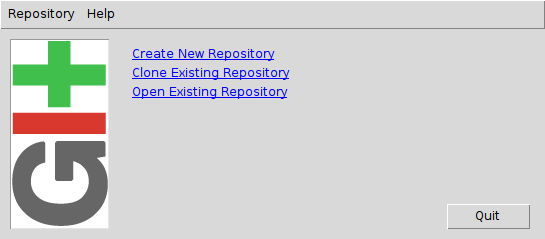
\includegraphics[scale=.6]{figuras/git-gui00-0}
  \item Selecione ``Clone Existing Repository'' (ou ``Clonar Repositório
    Existente''). Será criada uma janela como ilustrada abaixo.\\
    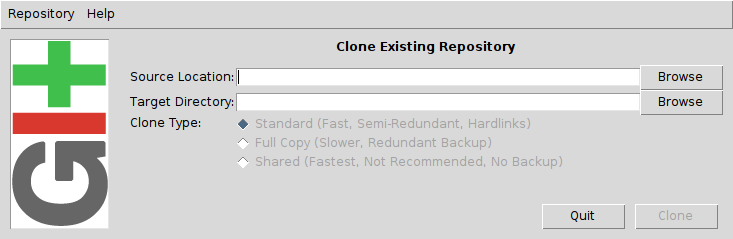
\includegraphics[scale=.6]{figuras/git-gui01}\\
  \item Preencha os campos ``Source Location'' (ou ``Endereço de Origem'') e
    ``Target Directory'' (ou ``Endereço de Destino''). O campo ``Source
    Location'' deve possuir exatamente o conteúdo da figura abaixo, i.e.,
    \url{https://github.com/r-gaia-cs/modelo_tese_imecc}, enquanto que ``Target
    Directory'' deve ser uma pasta a sua escolha (sugere-se utilizar o botão
    ``Browse'' ao lado do campo para fazer a seleção da pasta).\\
    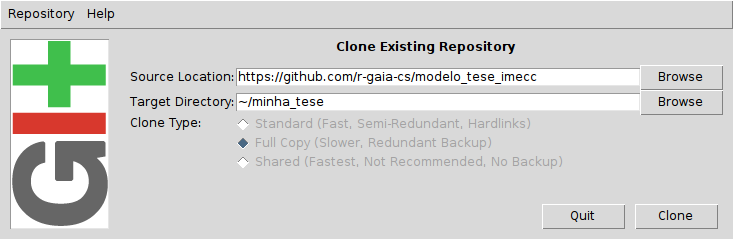
\includegraphics[scale=.6]{figuras/git-gui02}
  \item Depois de preencher os campos, pressione o botão ``Clone''. Irá aparecer
    uma janela mostrando o progresso de baixar o modelo e quando terminar
    basta pressione o botão ``Quit''.\\
    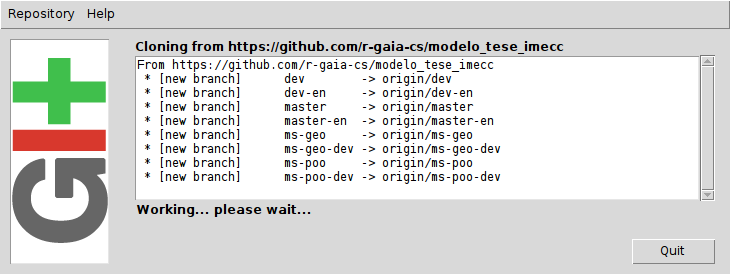
\includegraphics[scale=.6]{figuras/git-gui03}
\end{enumerate}

\subsection{Salvando modificações no modelo}
Modifique o modelo utilizando seu editor ou IDE favorito. Depois de realizar
algumas modificações siga os passos abaixo para salvar suas modificações.
\begin{enumerate}
  \item Inicialize o git-gui. Será criada uma janela como a ilustrada abaixo.\\
    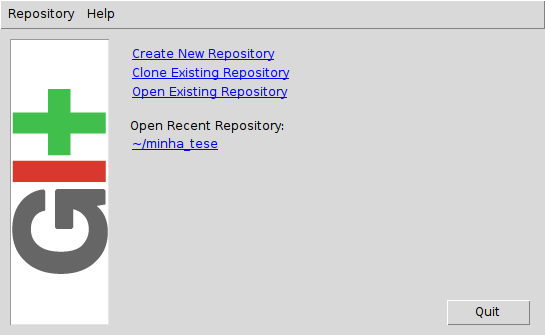
\includegraphics[scale=.6]{figuras/git-gui00-1}
  \item Se o endereço de onde salvou o modelo aparecer listado em ``Open Recent
    Repository'' (ou ``Repositórios Abertos Recentemente''), selecione-o. Caso
    contrário pressione ``Open Existing Repository'' (ou ``Abrir Repositório
    Existente'') e selecione a pasta do modelo. Será criada uma janela como a
    ilustrada abaixo.\\
    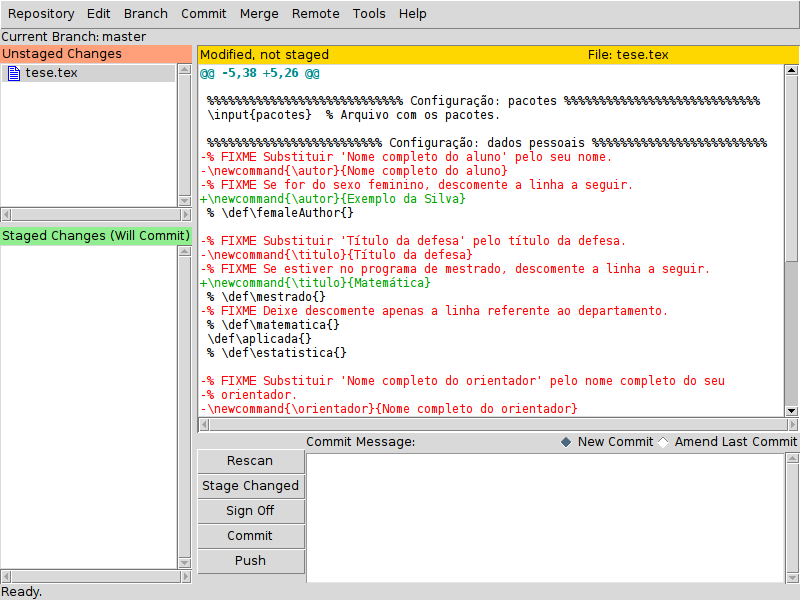
\includegraphics[scale=.6]{figuras/git-gui04-0}
  \item Partindo da barra de ferramentas no topo da janela, selecione
    \begin{itemize}
      \item \lstinline+Commit -> Rescan+,
      \item \lstinline+Commit -> Stage to Commit+,
      \item \lstinline+Commit -> Stage Changed Files to Commit+.
    \end{itemize}
    A janela terá sido modificada para algo próximo ao ilustrado abaixo.\\
    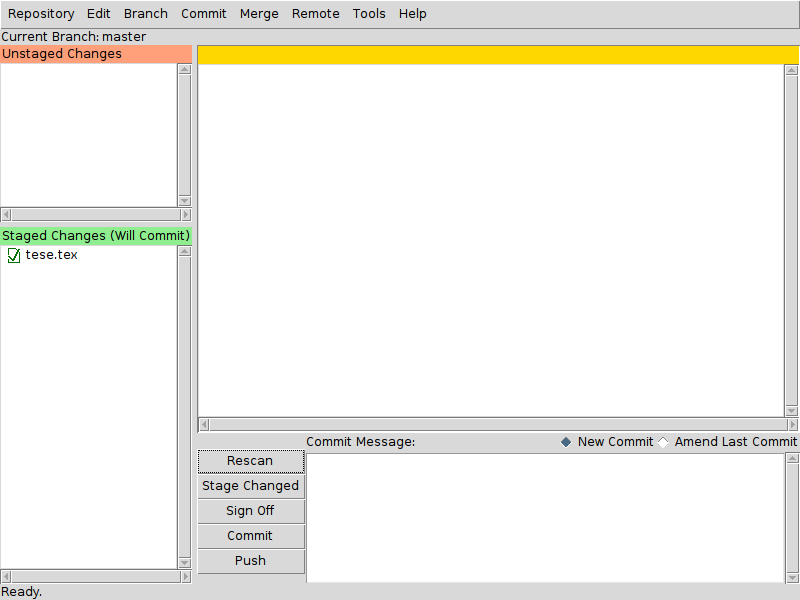
\includegraphics[scale=.6]{figuras/git-gui05}
  \item Digite um pequeno texto descrevendo as mudanças que fez na caixa de
    texto na parte de baixo da janela como ilustrado abaixo.\\
    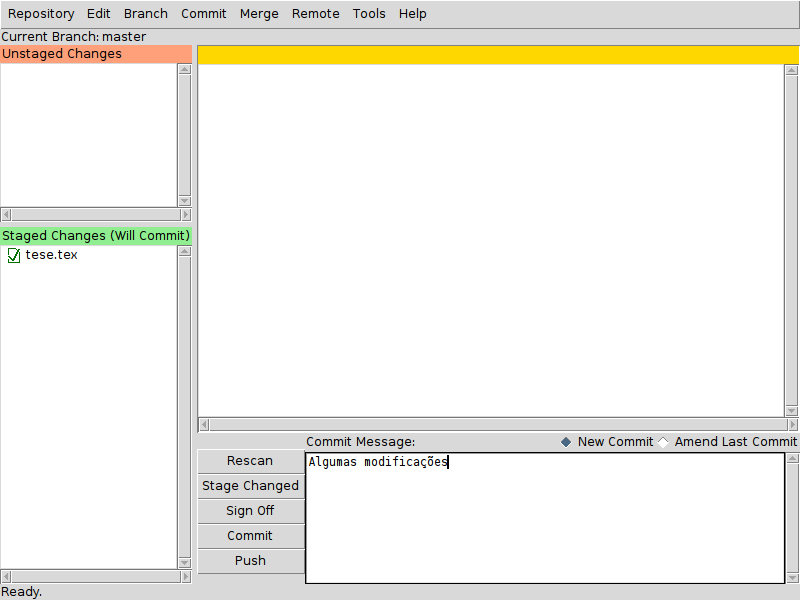
\includegraphics[scale=.6]{figuras/git-gui06}
  \item Ao lado da caixa de texto existe um botão ``Commit''. Pressione-o. A
    caixa de texto ficará em branco indicando que as modificações foram
    salvas.\\
    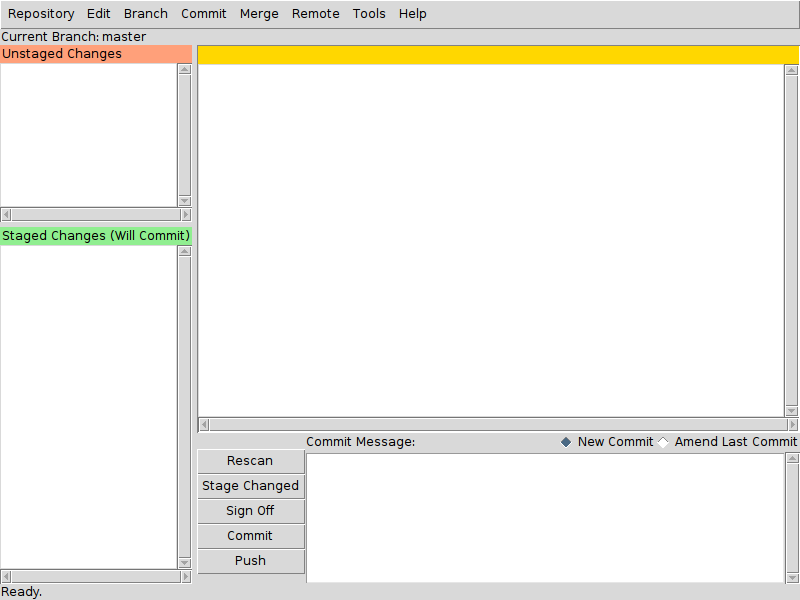
\includegraphics[scale=.6]{figuras/git-gui04-1}
\end{enumerate}

\subsection{Atualizando o modelo}
Como este modelo é um trabalho em progresso e não existe nenhuma garantia de que
as deliberações da Comissão Central de Pós-Graduação serão mantidas até que você
termine seu mestrado/doutorado é importante existir uma maneira de você
atualizar sua dissertação/tese já em processo de escrita com as novas
deliberações.

Uma vez salvo suas modificações como indicado na seção anterior, siga os passos
abaixo:
\begin{enumerate}
  \item Inicialize o git-gui. Será criada uma janela como a ilustrada abaixo.\\
    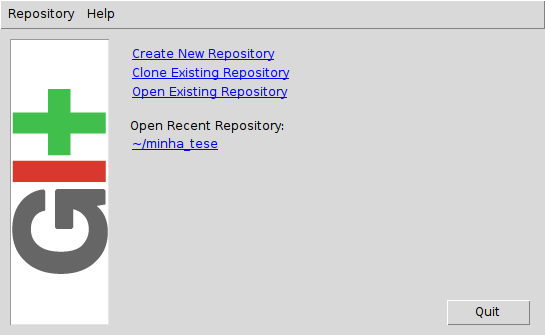
\includegraphics[scale=.6]{figuras/git-gui00-1}
  \item Se o endereço de onde salvou o modelo aparecer listado em ``Open Recent
    Repository'' (ou ``Repositórios Abertos Recentemente''), selecione-o. Caso
    contrário pressione ``Open Existing Repository'' (ou ``Abrir Repositório
    Existente'') e selecione a pasta do modelo. Será criada uma janela como a
    ilustrada abaixo.\\
    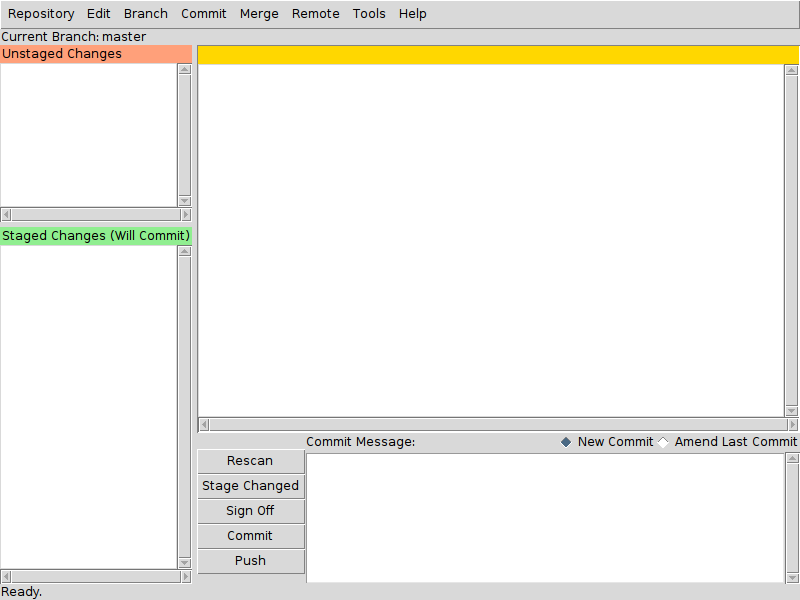
\includegraphics[scale=.6]{figuras/git-gui04-1}
  \item Partindo da barra de ferramentas no topo da janela, selecione
    \lstinline+Remote -> Fetch+ \lstinline+from -> origin+. Irá parecer uma janela
    mostrando o progresso de atualização do modelo. Se ao final do processo de
    atualização a janela for semelhante a\\
    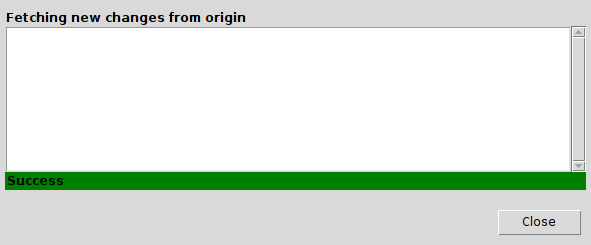
\includegraphics[scale=.6]{figuras/git-gui07-0}\\
    então você pode ignorar os passos a seguir. Já se a janela for semelhante
    a\\
    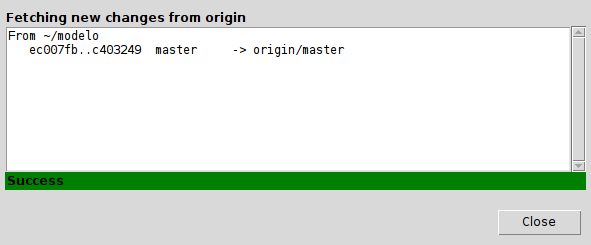
\includegraphics[scale=.6]{figuras/git-gui07-1}\\
    pressione o botão ``Close'' e prossiga com os passos abaixo.\\
  \item Partindo da barra de ferramentas no topo da janela, selecione
    \lstinline+Merge -> Local Merge+. Irá aparecer uma janela como ilustrada
    abaixo.\\
    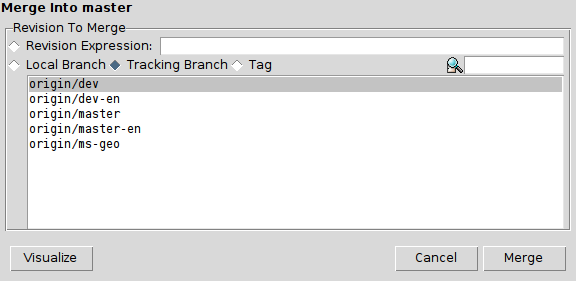
\includegraphics[scale=.6]{figuras/git-gui09}
  \item Selecione a opção \lstinline+origin/master+, como ilustrado abaixo, e
    pressione o botão ``Merge''.\\
    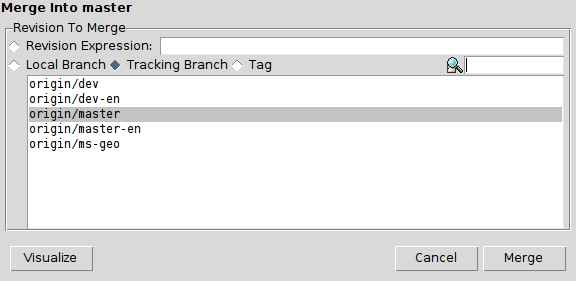
\includegraphics[scale=.6]{figuras/git-gui10}
  \item O seu trabalho seja atualizado com base no modelo e o resultado será
    mostrado em uma janela como ilustrado abaixo.\\
    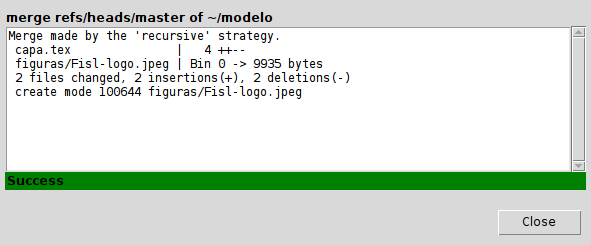
\includegraphics[scale=.6]{figuras/git-gui11}
\end{enumerate}
